\documentclass{article}
\usepackage{graphicx}
\graphicspath{ {./} }

\title{Homework 9, MTH 325}
\author{Thomas Bailey}
\date{November 2018}

\begin{document}
\maketitle

\begin{enumerate}
\item
  \begin{enumerate}
    \item A, Q, C, K, F, D, U, B, N, X, J, I, R, O, W, M, P
    \item A, V, L, I, F, T, R, E, C, O, N, M, D
    \item Y, F, O, X, Z, A, S, L, I, B, N, G, W, R, D, V, E
  \end{enumerate}
\item \addtocounter{enumi}{1}
  \begin{enumerate}
    \item A, Q, U, I, C, K, B, R, O, W, N, F, X, J, M, P, D
    \item A, V, L, F, T, E, C, N, M, D, O, R, I
    \item Y, F, O, I, B, V, E, X, Z, N, G, W, A, S, R, D, L
  \end{enumerate}
\item
  \begin{enumerate}
  \item
    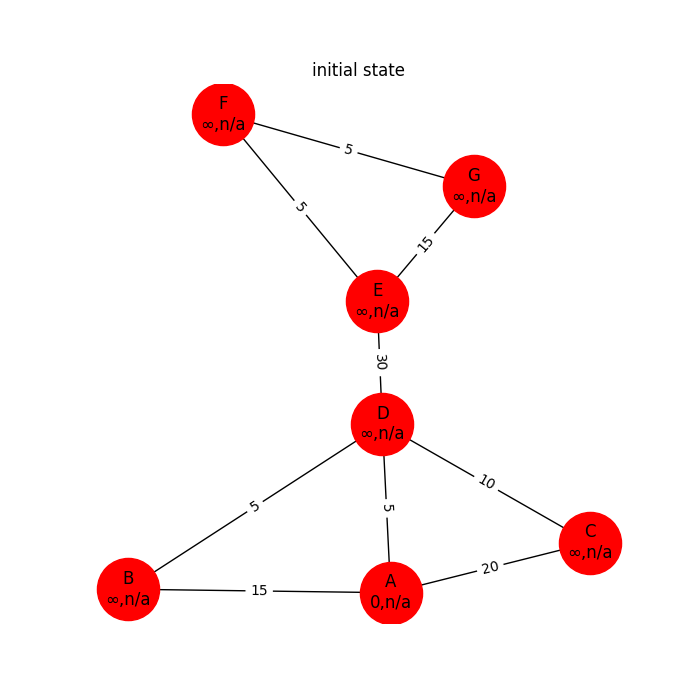
\includegraphics[width=\textwidth,height=\textheight,keepaspectratio]{4a0}
    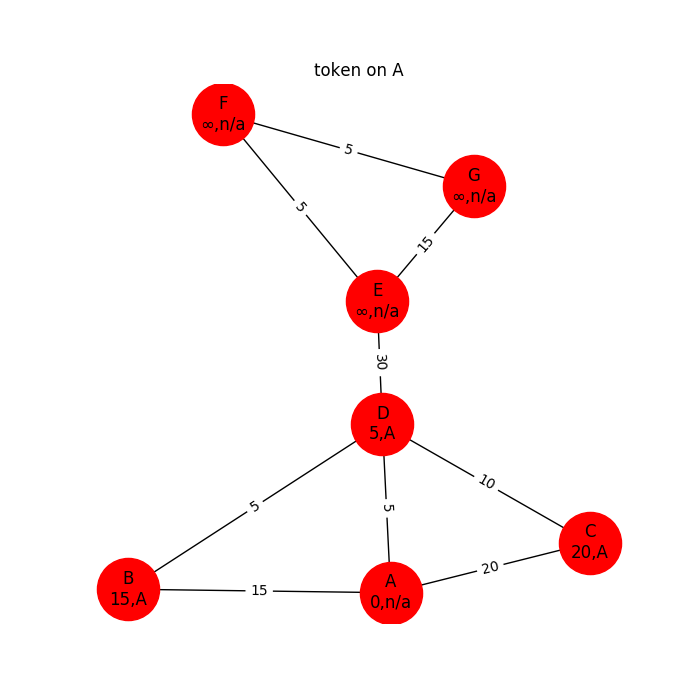
\includegraphics[width=\textwidth,height=\textheight,keepaspectratio]{4a1}
    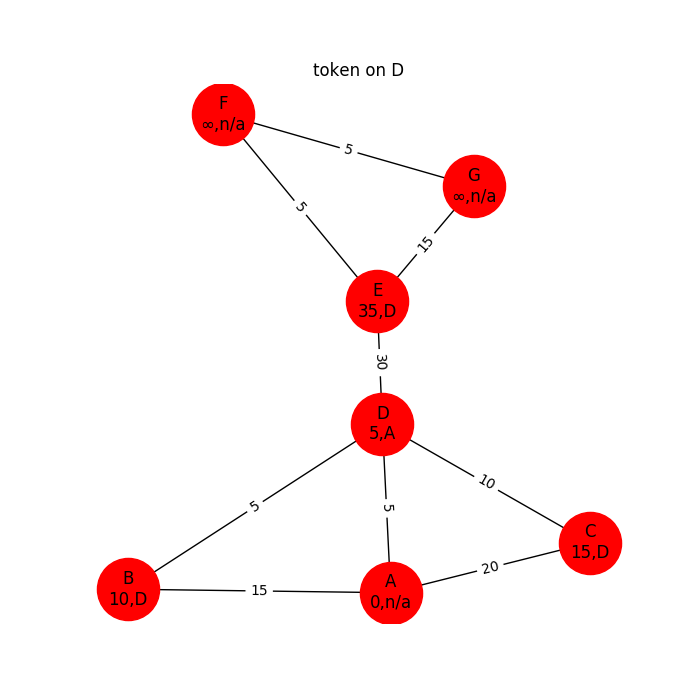
\includegraphics[width=\textwidth,height=\textheight,keepaspectratio]{4a2}
    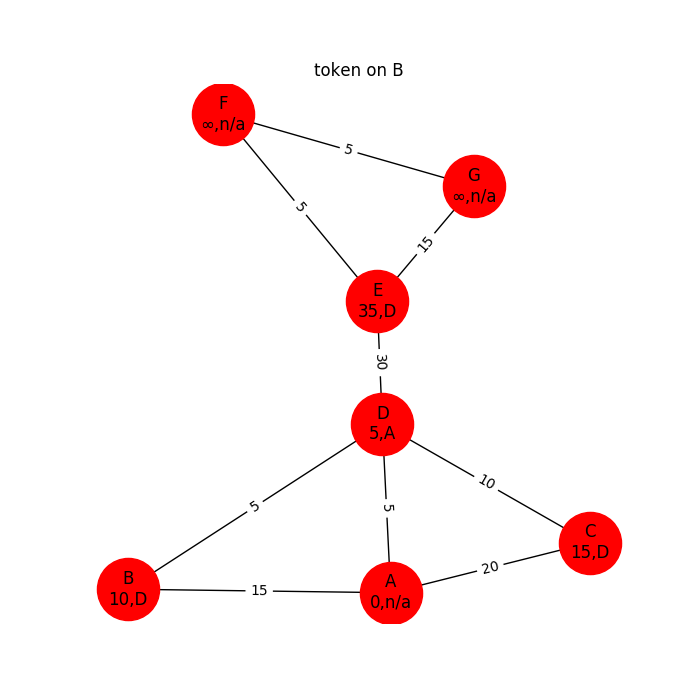
\includegraphics[width=\textwidth,height=\textheight,keepaspectratio]{4a3}
    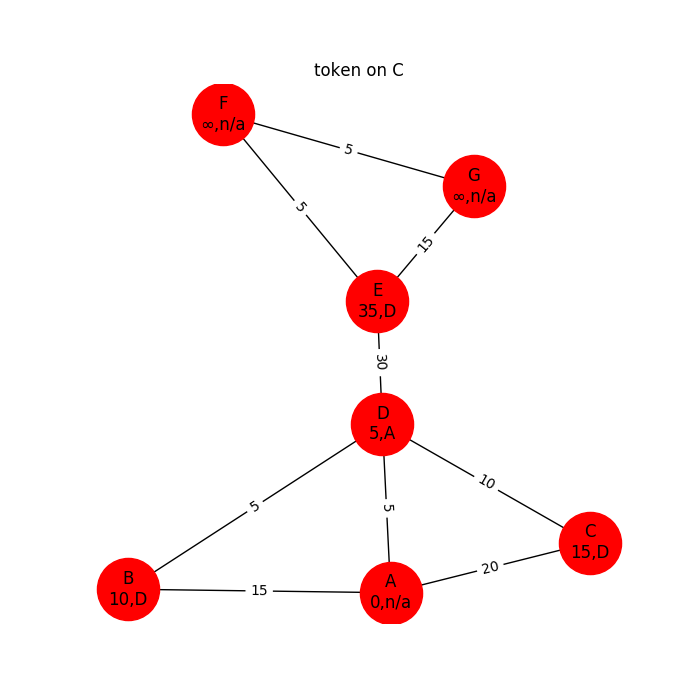
\includegraphics[width=\textwidth,height=\textheight,keepaspectratio]{4a4}
    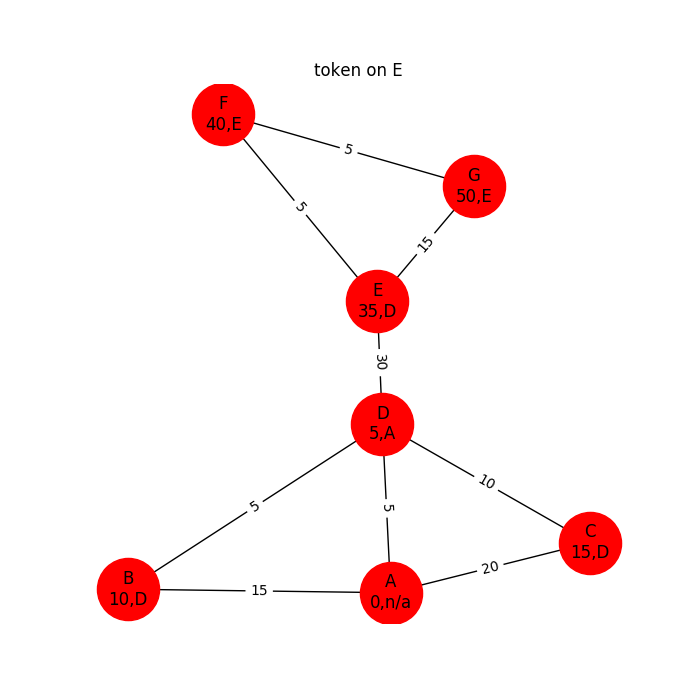
\includegraphics[width=\textwidth,height=\textheight,keepaspectratio]{4a5}
    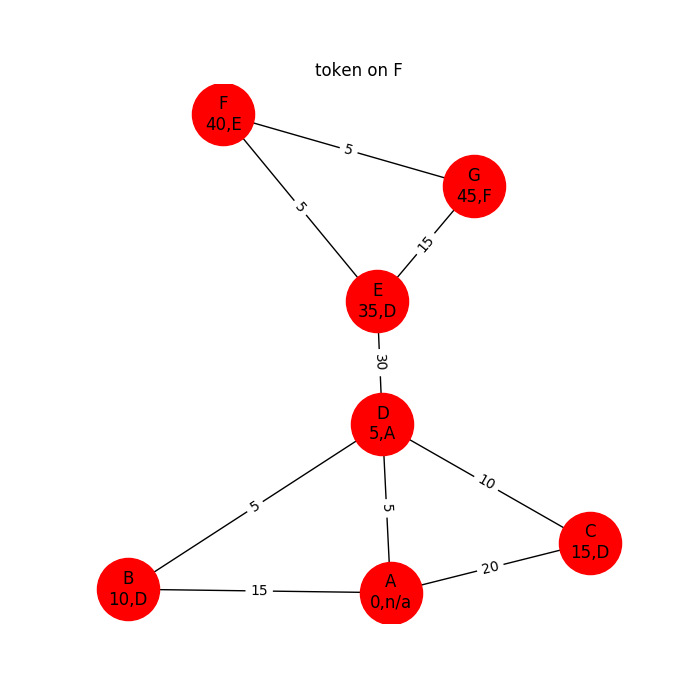
\includegraphics[width=\textwidth,height=\textheight,keepaspectratio]{4a6}
    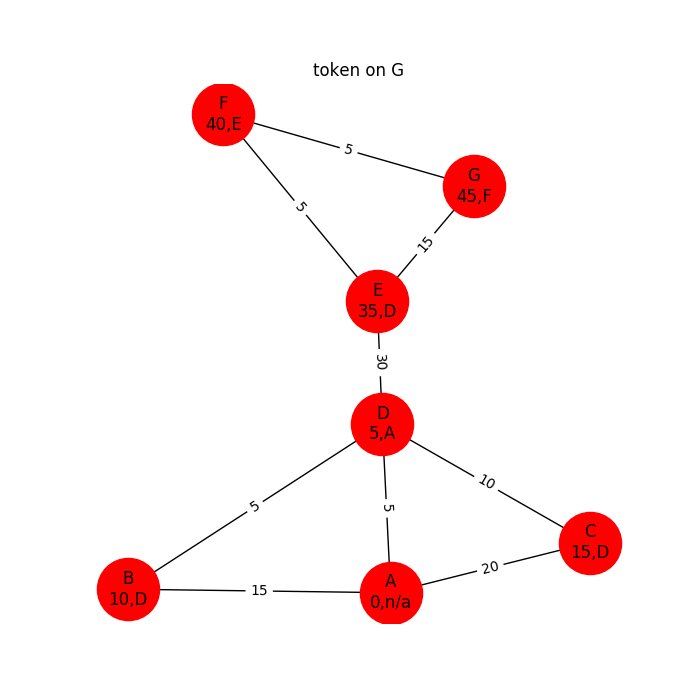
\includegraphics[width=\textwidth,height=\textheight,keepaspectratio]{4a7}
  \item
    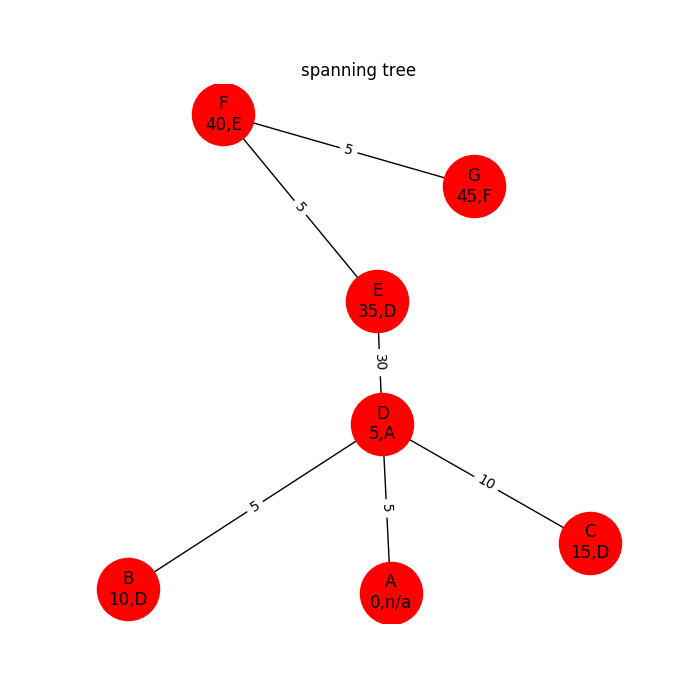
\includegraphics[width=\textwidth,height=\textheight,keepaspectratio]{4b}
  \item
    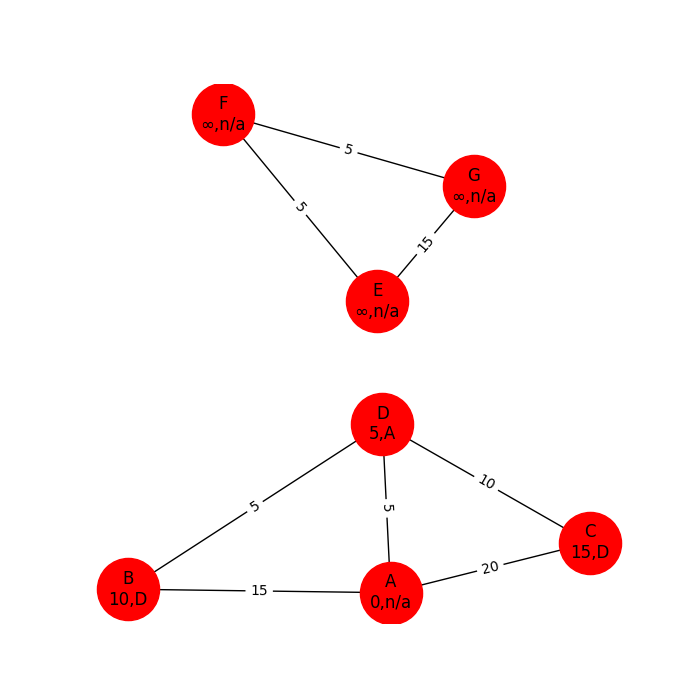
\includegraphics[width=\textwidth,height=\textheight,keepaspectratio]{4c}
  \end{enumerate}
\item
  \begin{enumerate}
  \item
    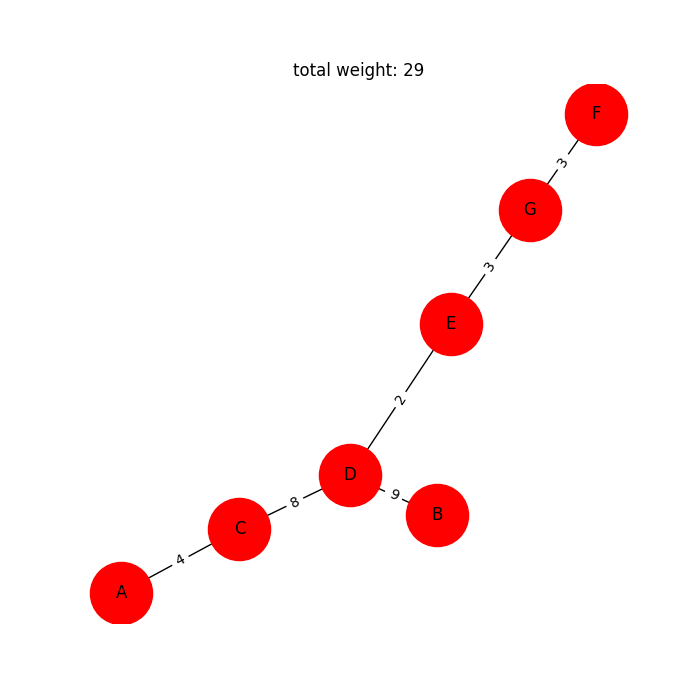
\includegraphics[width=\textwidth,height=\textheight,keepaspectratio]{5a}
  \item
    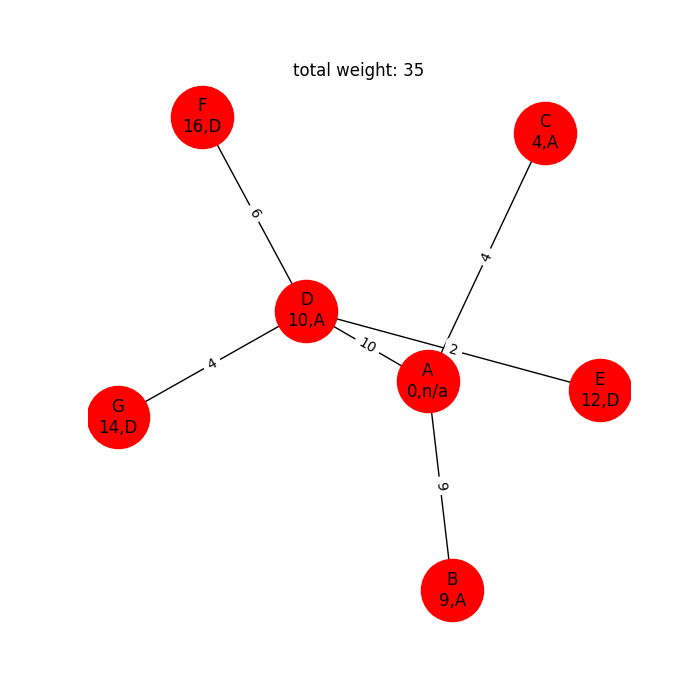
\includegraphics[width=\textwidth,height=\textheight,keepaspectratio]{5b}
  \item
    The edge $AD$ will never be part of a minimum spanning tree with A as the root because there is a better way to get from $A$ to $D$ through $C$. A minimum spanning tree is concerned with the overall minimum weight for the whole graph.
  \item
    The edge $AD$ will always be part of a minimum distance spanning tree with root $A$ because it is the shortest path from $A$ to $D$. The minimum distance spanning tree shows the shortest distance from any given point to the root, and does not minimize the total weight.
  \item
    Dijkystra's Algorithm does not also produce minimum spanning trees, and minimum distance spanning trees are not the same as minimum spanning trees.
  \end{enumerate}
  \end{enumerate}


\end{document}

